\chapter{Experimentaci\'on y Resultados}\label{chapter:resultados}
Todo el proceso de experimentaci\'on y los resultados logrados fueron por v\'ia del lenguaje de programaci\'on Python y sus bibliotecas. 

\section{Creaci\'on del corpus}

Para este problema, como bien se ha dicho, las investigaciones son casi nulas desde el punto de vista computacional, y como una de las consecuencias, no existen corpus grandes anotados, por ende fue necesario construir uno. 

En el trabajo con Aprendizaje Autom\'atico casi siempre la mirada gira en torno a la comparaci\'on entre los clasificadores y la b\'usqueda de las caracter\'isticas correctas para describir los elementos, y se asume que existe un juego de datos ideal para la corrida del algoritmo. Al menos este no ha sido el caso y evidencia lo complicada que es esta fase de la experimentaci\'on.

Inicialmente, se contaba con una pequeña muestra de tamaño 42, anotada por los ling\"uistas, con menos de 7 ejemplares por entonema. A partir de \'el se produjeron las grabaciones finales con un total de 271 audios, 7 a 27 muestras por clase y generados por un locutor de g\'enero femenino. La descripci\'on se muestra bien detallada en la Tabla \ref{Ta:tablita}. Es necesario no dejar pasar por alto lo ambig\"ua que llega a ser la anotaci\'on para alguien que no es especialista, puesto que como mismo algunos entonemas resultan inconfundibles, tales como el 6 y el 5b, por el papel tan especialmente expresivo que tienen en el habla coloquial de Cuba, otros no dejan l\'imites muy claros, tal es el caso de los entonemas 2 y 3 que expresan igualmente interrogaci\'on con alto grado de desconocimiento y deslindado solo por el tipo de respuesta, o tambi\'en, el caso del entonema 4, las preguntas que comienzan con \emph{Y}. La diferenciaci\'on de estas 3 categor\'ias, por ejemplo, es singularmente sutil desde un an\'alisis entonol\'ogico.

\begin{table}
\begin{center}
\begin{tabular}{l|r} \hline
\bf Entonema & \bf Cantidad de muestras \\ \hline
 1 & 25 \\ 
 1a & 16 \\ 
 1b & 27 \\ 
 1c & 18 \\ 
 2 & 14 \\ 
 2a & 23 \\ 
 3 & 26 \\ 
 3a & 15 \\ 
 3b & 7 \\
 4 & 11 \\
 4a & 17 \\
 5 & 12 \\
 5a & 11 \\
 5b & 10 \\
 6 & 10 \\
 6a & 10 \\
 7 & 7 \\
 7a & 12 \\ \hline
 
\end{tabular}
\caption{Muestras por entonema del corpus.}\label{Ta:tablita}
\end{center}
\end{table}




\subsection{Criterios para etiquetar el corpus}

Se consideraron los 18 entonemas estudiados e identificados por Garc\'ia River\'on. La anotaci\'on del corpus se produjo seg\'un las descripciones de la enton\'ologa para cada categor\'ia y con ayuda de las muestras iniciales para los casos menos evidentes.


\subsection{Aumento de datos} 
Puesto que 271 sigue siendo una cantidad pequeña para dar soluci\'on a este problema, fue necesario entonces el uso de \emph{aumento de datos}, lo cual se logr\'o por medio de la biblioteca \texttt{audiomentations}\footnote{\url{https://github.com/iver56/audiomentations}} de Python, aunque existen otras con la misma finalidad. De las transformaciones disponibles se aplicaron 14, que operan como las explicadas en \ref{aumento}.

\begin{comment}
\begin{enumerate}
\item TimeMask
\item FrequencyMask
\item AddGaussianSNR
\item PitchShift
\item TimeStretch
\item AddGaussianNoise
\item Shift
\item Shift without rollover
\item AddImpulseResponse
\item Resample
\item ClippingDistortion
\item AddBackgroundNoise
\item AddShortNoises
\end{enumerate}
\end{comment}


Para formar el conjunto \texttt{Test} se apartaron 2 de las grabaciones por entonema y las 14 transformaciones de cada uno, mientras que para el corpus final se conservaron las grabaciones restantes y el augmentation de 5 elegidas por entonema con 5 variantes por cada transformaci\'on. Se debe considerar que algunos de los audios aumentados fueron despreciados. Todas estas anotaciones quedan reflejadas con detalle en la tabla \ref{Ta:ct}.


\begin{table}
\begin{center}
\begin{tabular}{l|r|r} \hline
\bf Entonema & \bf Cant. muestras. Corpus. & \bf Cant. muestras. Conjunto Test \\ \hline
 1 & 371 & 30 \\ 
 1a & 363 & 28 \\ 
 1b & 372 & 30 \\ 
 1c & 365 & 30 \\ 
 2 & 361 & 29 \\ 
 2a & 367 & 28 \\ 
 3 & 372 & 30  \\ 
 3a & 362 & 30 \\ 
 3b & 355 & 29 \\
 4 & 355 & 29 \\
 4a & 363 & 30 \\
 5 & 357 & 30 \\
 5a & 355 & 30 \\
 5b & 356 & 30 \\
 6 & 354 & 30 \\
 6a & 356 & 30 \\
 7 & 350 & 29 \\
 7a & 355 & 29 \\ \hline
 Total & 6489 & 531 \\ \hline
\end{tabular}
\caption{Muestras por entonema del corpus final.}\label{Ta:ct}
\end{center}
\end{table}


\subsection{Vectorizaci\'on de la muestra}
Cada audio de entrada es caracterizado para su posterior clasificaci\'on por medio de:

\begin{description}
\item[cD:] Los coeficientes de detalle de la curva mel\'odica en el nivel 4 de descomposici\'on de la Transformada Wavelet Discreta con la base wavelet \emph{Daubechies}\cite{daubechies1992cbms}. En promedio, para los audios del corpus, tienen tama\~no 40.
\item[espectrum:] El espectro de potencias de la curva. Tiene dimensi\'on 300 en promedio.
\item[pendiente:] La pendiente del \emph{pitch} en s\'i mismo. Es un escalar.
\item[entrop\'ia:] Se consideran la del \emph{pitch} y la de los coeficientes de detalle.
\item[convoluci\'on:] Convoluci\'on linear discreta entre la curva mel\'odica y la reconstrucci\'on de la misma que se logra con los \emph{cD} del primer nivel en la descomposici\'on con DWT. Es un escalar\footnote{El primer valor de aplicar \texttt{scipy.signal.convolve()} como se explica en las \emph{Especificaciones de la implementaci\'on}.}.
\item[frecuencias:] Se consideran la frecuencia m\'axima, m\'inima, inicial y final de la curva mel\'odica. Estas caracter\'isticas son para representar el rasgo de \emph{registro}, se\~nalado por Garc\'ia River\'on.
\end{description}

\subsection{Peque\~nas especificaciones sobre la implementaci\'on}
La implementaci\'on fue desarrollada completamente con el lenguaje de programaci\'on Python:

\begin{enumerate}
\item Las grabaciones de los entonemas se codificaron en formato \texttt{.wav}.

\item La extracci\'on de la curva mel\'odica de cada segmento de audio se produjo con \texttt{amfm\_decompy.pYAAPT()}\footnote{\url{https://pypi.org/project/AMFM-decompy/}} que es una versi\'on para Python del algoritmo descrito en \emph{Yet Another Algorithm for Pitch Tracking} \cite{kasi2002yet}.

\item El trabajo con wavelets se desarroll\'o con \texttt{pyw}\footnote{\url{https://pywavelets.readthedocs.io/en/latest/}}: la DWT espec\'ificamente con, \texttt{pyw.dwt()} y la reconstrucci\'on de la se\~nal a partir de los coeficientes de detalles y de aproximaci\'on de cierto nivel, con \texttt{pyw.waverec()}.

\item La transformada discreta de Fourier se obtuvo con \texttt{numpy.fft.fft()}. Para hallar el espectro se utiliz\'o la variante de los m\'odulos.

\item La entrop\'ia se calcul\'o con un m\'etodo simple implementado por el autor.

\item La pendiente se determin\'o por medio de \texttt{numpy.polyfit()}.

\item El valor de convoluci\'on es el primero de la muestra discreta de tama\~no 2 que devuelve \texttt{scipy.signal.convolve()} con el par\'ametro \texttt{mode = "valid"}.

\item La manipulaci\'on y almacenamiento de los datos se produjo con \texttt{pandas}\footnote{\url{https://pandas.pydata.org/}}.

\item Todo el trabajo con Aprendizaje Autom\'atico se desarroll\'o con \texttt{sklearn} \cite{garreta2013learning}: los clasificadores SVM y regresi\'on log\'istica con \texttt{sklearn.svm.SVC} y \texttt{sklearn.linear\_model.LogisticRegression} y para el an\'alisis de los modelos se emple\'o \texttt{sklearn.model\_selection} y \texttt{sklearn.metrics}. 
\end{enumerate}






\subsection{Preprocesamiento}
Para la extracci\'on de caracter\'isticas de la curva mel\'odica se experimentaron dos preprocesamientos fundamentales:

\begin{description}
\item[Remover silencios:] Eliminar los valores iguales a cero del inicio y final de la curva.
\item[Corregir discontinuidad:] Se rellenan los silencios intermedios del \emph{pitch} estimando los valores que tomar\'ia si fuesen distintos de cero por medio de interpolaci\'on. 
\end{description}

Los resultados expuestos en la siguiente secci\'on solo tienen aplicado el primero de estos preprocesamientos, puesto que el segundo luce muy prometedor, pero en la pr\'actica solo reduce la puntuaci\'on de los clasificadores.

\section{Resultados}
Los clasificadores que esencialmente se aplicaron fueron \emph{SVM} y \emph{Regresi\'on Log\'istica}. Para estimar el sesgo y la varianza de cada clasificador se aplic\'o validaci\'on cruzada\footnote{Los resultados expuestos se produjeron con \texttt{sklearn.model\_selection.ShuffleSplit}~ (\url{https://scikit-learn.org/stable/modules/generated/sklearn.model_selection.ShuffleSplit.html})} con raz\'on de $60\%$ para entrenar $40\%$ para validar y 30 repeticiones. Las curvas de aprendizaje\cite[secci\'on 7.5.4]{murphy2012machine} sirvieron para detectar la presencia o no de \emph{overfitting} \cite[p.22]{murphy2012machine}.

\subsection{Experimento 1}
Las muestras de audio fueron vectorizadas 
considerando todas las cararacter\'isticas 
descritas 
en la secci\'on anterior. Los 
resultados\footnote{Los modelos fueron validados
 atendiendo a la 
medida accuracy y la varianza\cite{murphy2012machine}.} 
se reflejan en la Tabla \ref{r1} y 
las curvas de aprendizaje en las Figuras \ref{calr1} y \ref{casvm1}.



\subsection{Experimento 2}
Los audios se vectorizaron igualmente que como en el experimento 1, excepto que se prescindi\'o de los valores del espectro, por tanto se alcanza una reducci\'on considerable de la dimensi\'on del problema\footnote{De 433 caracter\'isticas se comienza a trabajar solo con 41.} para tratar de evadir el efecto de \emph{overfitting}. Los resultados se reflejan en la Tabla \ref{r2} y las curvas de aprendizaje en las Figuras \ref{carl2} y \ref{casvm2}.


\begin{figure}
\begin{center}
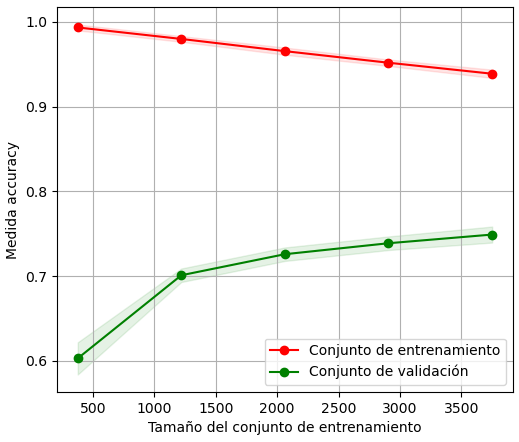
\includegraphics[width= 0.5\columnwidth]{Graphics/1}
\caption{Curva de aprendizaje con Regresi\'on Log\'istica. Experimento 1.}
\label{calr1}
\end{center}
\end{figure}

\begin{figure}
\begin{center}
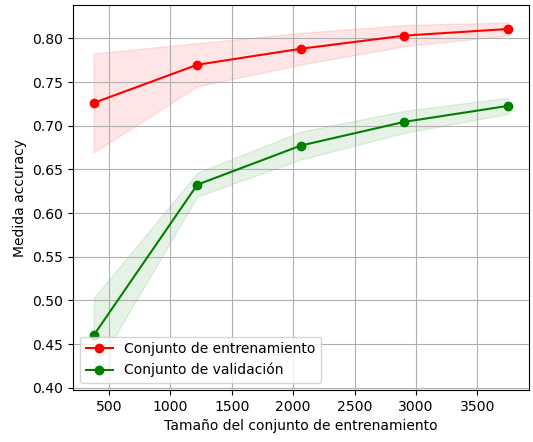
\includegraphics[width= 0.5\columnwidth]{Graphics/2}
\caption{Curva de aprendizaje con SVM. Experimento 1.}
\label{casvm1}
\end{center}
\end{figure}

\begin{table}
\begin{center}
\begin{tabular}{l|r|r} 
   & \bf Medida accurracy & \bf Varianza \\ \hline
 \bf SVM & 0.72 & 0.01 \\ 
 \bf Regresi\'on Log\'istica & 0.74 & 0.01 \\ 
\end{tabular}
\caption{Resultados de la validaci\'on cruzada. Experimento 1.}\label{r1}
\end{center}
\end{table}

\begin{figure}
\begin{center}
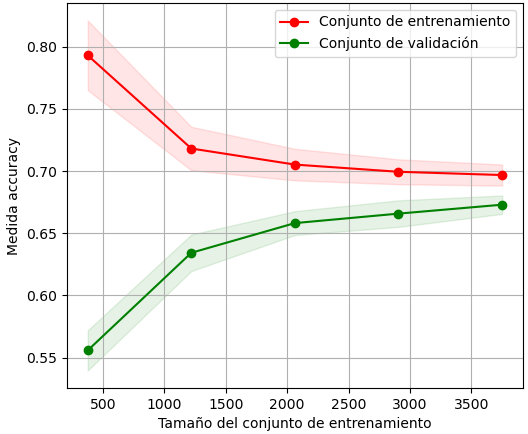
\includegraphics[width= 0.5\columnwidth]{Graphics/3}
\caption{Curva de aprendizaje con Regresi\'on Log\'istica. Experimento 2.}
\label{carl2}
\end{center}
\end{figure}

\begin{figure}
\begin{center}
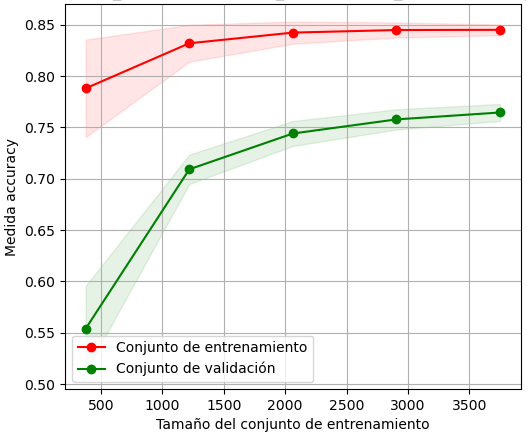
\includegraphics[width= 0.5\columnwidth]{Graphics/4}
\caption{Curva de aprendizaje con SVM. Experimento 2.}
\label{casvm2}
\end{center}
\end{figure}

\begin{table}
\begin{center}
\begin{tabular}{l|r|r} 
   & \bf Medida accurracy & \bf Varianza \\ \hline
 \bf SVM & 0.76 & 0.01 \\ 
 \bf Regresi\'on Log\'istica & 0.67 & 0.01 \\ 

\end{tabular}
\caption{Resultados de la validaci\'on cruzada. Experimento 2.}\label{r2}
\end{center}
\end{table}

\subsection{Evaluaci\'on en el conjunto \texttt{Test}}
Se elige el clasificador SVM del Experimento 2, pues presenta mayor puntaci\'on, su curva no indica presencia de \emph{overfitting} y considera menos caracter\'isticas. Los resultados\footnote{El an\'alisis se produjo antendiendo a la presici\'on, el recobrado y la medida-f1\cite{murphy2012machine,bay2009evaluation}.} de su evaluaci\'on en el conjunto \texttt{Test} se muestran en la Tabla \ref{test_result} y la Figura \ref{mcsvm2}. Se observa que la predicci\'on es nula para los entonemas VE-2a, VE-3a, E-5, VE-5a, VE-5b y E-6. Aunque no son buenas noticias, no indica necesariamente que el modelo sea incapaz siempre de predecir correctamente estas categor\'ias, recordando que, el conjunto \texttt{Test} es el \emph{Data Augmentation} de solo dos ejemplos por entonema.
\begin{table}
\begin{center}
\begin{tabular}{l|rrrr} 
& \bf precisi\'on & \bf recobrado & \bf medida-F1 & \bf   cantidad \\ \hline
         \bf 1 &       0.39  &    0.83  &    0.53   &     30 \\ 
         \bf 1a  &     0.16  &    0.32  &    0.21  &      28 \\
         \bf 1b    &   0.30   &   0.77 &     0.43    &    30 \\
         \bf 1c  &     0.52   &   0.80   &   0.63    &    30 \\
         \bf  2    &   0.17   &   0.14   &   0.15   &     29 \\
         \bf 2a     &  0.00  &    0.00   &   0.00    &    28 \\
        \bf   3   &    0.43  &   0.30  &    0.35  &      30 \\
        \bf  3a  &     0.00 &   0.00  &    0.00  &      30 \\
         \bf  3b  &     0.44 &   0.66  &    0.53    &    29 \\
       \bf   4   &    0.09  &   0.14  &    0.11     &   29 \\
       \bf  4a  &    0.23  &   0.10  &    0.14     &   30 \\
      \bf  5   &    0.00  &   0.00  &    0.00      &  30 \\
      \bf  5a  &     0.00 &   0.00  &    0.00     &   30 \\ 
     \bf   5b  &     0.00 &   0.00  &    0.00     &   30 \\
    \bf    6     &  0.00    &  0.00   &   0.00   &     30 \\
    \bf  6a     &  0.14    &  0.10   &   0.12    &    30 \\
     \bf    7     &  0.31    &  0.17   &   0.22     &   29 \\
   \bf  7a     &  0.57    &  0.45   &   0.50     &   29 \\ \hline
          \bf Medida accuracy     &          &         &  0.27     &  531 \\

\end{tabular}
\caption{Evaluaci\'on en el conjunto \texttt{Test}. Experimento 2. SVM.}\label{test_result}
\end{center}
\end{table}

\begin{figure}
\begin{center}
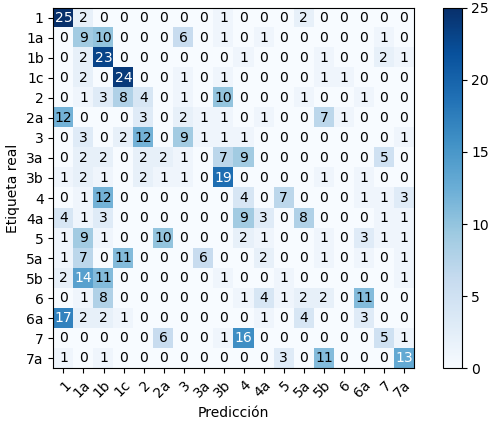
\includegraphics[width= 0.5\columnwidth]{Graphics/5}
\caption{Matriz de confusi\'on. Evaluado en conjunto \texttt{Test}. SVM Experimento 2.}
\label{mcsvm2}
\end{center}
\end{figure}

\begin{comment}
Raquel dice:
Segun estos indicadores, se pudo comprobar que las variantes VE-Ia, VE-lc, VE-2a, VE-3a. VE-3b y RE-6a se diferencian par un rasgo unico: la forma. Se ha observado que el rasgo mas productiv~ en este sentido es precisamente la forma del contamo mel6dico. 
- el diapason es importante
\end{comment}


\section{Software}
El producto final es un software que grafica el espectrograma de un audio de entrada y predice el entonema presente. La interfaz gr\'afica se produjo con la biblioteca \texttt{PyQt5} de Python y est\'a reflejada en las Figuras \ref{software} y \ref{software2} de los anexos.